\section{Kravspecifikation}
\subsection{Beskrivelse}
Det endelige system er en sikker meddelelsesplatform, hvori man kan sende og modtage beskeder over et socialt medie, derfor har gruppen tænkt følgende use-case forløb, som et udgangspunkt.

\begin{table}[H]
    \begin{minipage}{.5\textwidth}
        \begin{figure}[H]
            \centering
            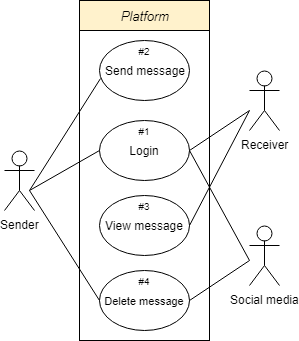
\includegraphics[width=0.85\linewidth]{Projectdoc/Assets/Illustrationer/simple-usecase.png}
            \caption{Usecase diagram}
            \label{fig:usecase}
        \end{figure}
    \end{minipage}
    \begin{minipage}{.5\textwidth}
        \textbf{Herved kan vi definere de givende hovedfunktioner:}
        \begin{itemize}
            \item Brugere skal kunne logge ind i systemet, for betjening.
            \item Systemets sendte beskeder skal deles igennem et socialt medie.
            \item Sendte beskeder skal formateres, for bevarelse af brugerenes sikkerhed.
            \item Systemet skal kunne vise / genindlæse tidligere sendte beskeder.
            \item Brugere skal i systemet kunne slette deres tidligere afsendte beskeder.
        \end{itemize}
    \end{minipage}
\end{table}

Given denne overstående beskrivelse kan der i alt formuleres to forskellige hovedscenarier for produktets anvendelse, der begge definerer produktets endelige mål.
\subsubsection{Usecase: Send besked}
\label{Hovedscenarie1}
For forsendelse, af beskeder gennem produktet, vil brugeren skulle først udføre usecase \#1. "Login" [\ref{Usecase1_Login}]. Denne usecase vil registre brugeren til senere genkendelse, for f.eks. muligheden til redigering, eller at slette deres oprettede besked tråde eller enkelte posts. Brugeren kan dog også vælge at foretage en såkaldt anonym registration, hvor brugren ikke selv direkte sættes i sammenhæng med den postede besked, men i stedet er blevet formidlet igennem en fælles talsperson registreret af produktet selv. Efterfølgende vil brugeren skulle udføre usecase \#2. "Send message" [\ref{Usecase2_Send_Message}], hvor brugeren blandt andet vil få mulighed for at vælge f.eks. en specifik sammenhæng hvori brugerens besked vil blive kædet sammen. Det bagved læggende system vil håndtere kryptering af beskedens tekst, og dens indarbejdelse i en steganografisk sammenhæng, og vil efterfølgende også gennem API strukturer, udgive den nedskrevne besked til det aktuelle sociale medie.
\subsubsection{Usecase: Se beskeder}
\label{Hovedscenarie2}
For fremvisning af beskeder i produktet, vil brugeren som i forgående hovedscenarie [\ref{Hovedscenarie1}] først skulle udføre usecase \#1. "Login". Efter denne skal brugeren gennemgå usecase \#3 "View message" [\ref{Usecase3_View_Message}], hvor brugeren vil blive præsenteret med muligheden for at vælge, først en specifik tråd, hvori der kan forekomme en række af flere enkelte beskeder, og efterfølgende f.eks. en længere enkelt stående tekst besked.
Selvfølgelig er denne omtalte tråd og tekst repræsentation ikke fremvist under steganografi, men er blevet bearbejdet af systemet til at være læselig.
Endvidere under disse fremvisninger, kan en bruger også vælge at slette en besked eller hele tråde, såfremt at brugeren har registreret ejerskab over disse.

\subsection{Krav}
\begin{itemize}
    \item \textbf{Funktionelle krav}
    \begin{itemize}
        \item Systemet skal kunne sende beskeder/indlæg.
        \item Systemet skal kunne vise beskeder/indlæg.
        \item Beskeder skal lagres på et socialt medie.
        \item Lagerede beskeder skal være skjult via steganografi.
        \item Systemet skal foretage kommunikationen anonymt.
    \end{itemize}
    \item \textbf{Ikke-funktionelle krav}
    \begin{itemize}
        \item Brugere skal kunne slette tidligere sendte beskeder.
        \item Beskeder skal kunne kædes i længere sammenhæng.
        \item Det må ikke forekomme indstillinger der forværrer brugerens sikkerhed.
        \item 80\% af testbrugerne skal kunne navigere systemet uden yderligere instruktioner.
        \item Systemet skal præsentere beskeder på en overskuelig måde.
        \item Systemet må ikke udelukkende sikres med steganografi.
    \end{itemize}  
\end{itemize}

%- Design krav:
%- Visuelt "Sikkert at bruge"
%- Få, men detaljeret posts
%- Farver udståler trykhed og tillid.½